\documentclass{article}
\usepackage[utf8]{inputenc}
\usepackage{caratula}
\usepackage{minted}

\usepackage{graphicx}
\usepackage{verbatim}
\usepackage{amsmath}
\usepackage{multirow}
\usepackage{multicol}
\usepackage{a4wide}
\usepackage{rotating}
\usepackage[shortlabels]{enumitem}
\usepackage{caratula}
\usepackage[spanish]{babel}

\usepackage{hyperref}
\hypersetup{
	colorlinks=true,
	linkcolor=blue,
	filecolor=magenta,      
	urlcolor=blue,
}

% \title{}
% \author{  \\ Ezequiel Reiner \\ Natalia Pesaresi}
% \date{July 2018}
\usemintedstyle{friendly}    


\begin{document}

\thispagestyle{empty}
\materia{Teoria de Lenguajes}
\submateria{Primer Cuatrimestre de 2018}
\titulo{Conversor de JSON a YAML}
%\subtitulo{Procesamiento de imágenes}

\integrante{Regnier, Ezequiel}{836/13}{eze\_regnier@hotmail.com}
\integrante{Zamboni, Gianfranco}{219/13}{gianfranco376@gmail.com}
\integrante{Pesaresi, Natalia}{636/14}{natalia.pesaresi@gmail.com}

\maketitle

\newpage

\tableofcontents
\newpage

\section{Introducción}

En este trabajo, se propone realizar un conversor de código JSON a código YAML. Como ambos lenguajes poseen las mismas estructuras, la conversión solo implica formatear correctamente la cadena de entrada para que su sintaxis sea acorde a la cadena de salida. \\ \\
Por ejemplo en el caso de los arrays: \\

\begin{center}
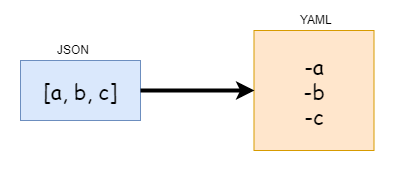
\includegraphics[scale=0.7]{img1.png}
\end{center}

Para realizar esta conversión, se necesitará un Lexer que reconozca las cadenas que pertenecen al lenguaje JSON. Y un parser que traduzca sintácticamente la escritura a YAML.

\section{Gramática}
Para implementar el traductor, se decidio usar la librería ply, una herramienta de python que utilizas grámaticas LR para generarlo. Por lo que la grámatica diseñada, además de generar el lenguaje descripto en la especificación de JSON, debe cumplir con este requisito.

Se propone:

\begin{align*}
G=< \{Value, Object, Array, Members, Pair, Elements\}, \\ \{\texttt{string}, \texttt{number}, \texttt{true}, \texttt{false}, \texttt{null}, \texttt{[}, \texttt{]}, \texttt{\{}, \texttt{\}}, \texttt{:} \}, Value, P>
\end{align*}
Donde P es:

\begin{multicols}{2}
			\setlist{start=0}
	\begin{enumerate}[(1)]
		\item $S' \to Value$\hspace*{5mm}
		\item $Value \to Object$
		\item $Value \to Array$
		\item $Value \to \texttt{string}$
		\item $Value \to \texttt{number}$
		\item $Value \to \texttt{true}$
		\item $Value \to \texttt{false}$
		\item $Value \to \texttt{null}$
		\item $Object \to \texttt{\{ \}}$
		\item $Object \to \texttt{\{} Members \texttt{\}}$
		\item $Members \to Pair$
		\item $Members \to Pair \texttt{,} Members$
		\item $Pair \to \texttt{string :} Value$
		\item $Array \to \texttt{[ ]}$
		\item $Array \to \texttt{[} Elements \texttt{]}$
		\item $Elements \to Value$
		\item $Elements \to Value \texttt{,} Elements$
	\end{enumerate}
\end{multicols}


Para verificar que efectivamente esta es una grámatica LR, se usó la herramienta \textit{LALR(1) Parser Generator} [-1-] para generar las tablas LR de acción y goto y verificar, de esta forma, que no haya conflictos.
\begin{sidewaysfigure}
\caption{LR Table}
\begin{center}
\begin{tabular}{ |c|c|c|c|c|c|c|c|c|c|c|c|c|c|c|c|c|c|c|c|c|c|c| }
			\hline
			\multirow{2}{*}{\textbf{State}}  & \multicolumn{12}{|c|}{\textbf{ACTION}} & \multicolumn{7}{|c|}{\textbf{GOTO}}\\
			\cline{2-20}
			 & \texttt{string} & \texttt{number} & \texttt{true} & \texttt{false} &\texttt{null} & \{ & \} & \texttt{,} & \texttt{:} & \texttt{[} & \texttt{]} & \texttt{\$} & $S'$ & $Value$ & $Object$ & $Members$ & $Pair$ & $Array$ & $Elements$ \\ \hline
			0 & S4 & S5 & S6 & S7 & S8 & S9 &   &   &   & S10 &   &   &   & 1 & 2 &   &   & 3 &  \\ \hline 
			1 &   &   &   &   &   &   &   &   &   &   &   & Acc &   &   &   &   &   &   &  \\ \hline 
			2 &   &   &   &   &   &   & R1 & R1 &   &   & R1 & R1 &   &   &   &   &   &   &  \\ \hline 
			3 &   &   &   &   &   &   & R2 & R2 &   &   & R2 & R2 &   &   &   &   &   &   &  \\ \hline 
			4 &   &   &   &   &   &   & R3 & R3 &   &   & R3 & R3 &   &   &   &   &   &   &  \\ \hline 
			5 &   &   &   &   &   &   & R4 & R4 &   &   & R4 & R4 &   &   &   &   &   &   &  \\ \hline 
			6 &   &   &   &   &   &   & R5 & R5 &   &   & R5 & R5 &   &   &   &   &   &   &  \\ \hline 
			7 &   &   &   &   &   &   & R6 & R6 &   &   & R6 & R6 &   &   &   &   &   &   &  \\ \hline 
			8 &   &   &   &   &   &   & R7 & R7 &   &   & R7 & R7 &   &   &   &   &   &   &  \\ \hline 
			9 & S14 &   &   &   &   &   & S11 &   &   &   &   &   &   &   &   & 12 & 13 &   &  \\ \hline 
			10 & S4 & S5 & S6 & S7 & S8 & S9 &   &   &   & S10 & S15 &   &   & 17 & 2 &   &   & 3 & 16\\ \hline 
			11 &   &   &   &   &   &   & R8 & R8 &   &   & R8 & R8 &   &   &   &   &   &   &  \\ \hline 
			12 &   &   &   &   &   &   & S18 &   &   &   &   &   &   &   &   &   &   &   &  \\ \hline 
			13 &   &   &   &   &   &   & R10 & S19 &   &   &   &   &   &   &   &   &   &   &  \\ \hline 
			14 &   &   &   &   &   &   &   &   & S20 &   &   &   &   &   &   &   &   &   &  \\ \hline 
			15 &   &   &   &   &   &   & R13 & R13 &   &   & R13 & R13 &   &   &   &   &   &   &  \\ \hline 
			16 &   &   &   &   &   &   &   &   &   &   & S21 &   &   &   &   &   &   &   &  \\ \hline 
			17 &   &   &   &   &   &   &   & S22 &   &   & R15 &   &   &   &   &   &   &   &  \\ \hline 
			18 &   &   &   &   &   &   & R9 & R9 &   &   & R9 & R9 &   &   &   &   &   &   &  \\ \hline 
			19 & S14 &   &   &   &   &   &   &   &   &   &   &   &   &   &   & 23 & 13 &   &  \\ \hline 
			20 & S4 & S5 & S6 & S7 & S8 & S9 &   &   &   & S10 &   &   &   & 24 & 2 &   &   & 3 &  \\ \hline 
			21 &   &   &   &   &   &   & R14 & R14 &   &   & R14 & R14 &   &   &   &   &   &   &  \\ \hline 
			22 & S4 & S5 & S6 & S7 & S8 & S9 &   &   &   & S10 &   &   &   & 17 & 2 &   &   & 3 & 25\\ \hline 
			23 &   &   &   &   &   &   & R11 &   &   &   &   &   &   &   &   &   &   &   &  \\ \hline 
			24 &   &   &   &   &   &   & R12 & R12 &   &   &   &   &   &   &   &   &   &   &  \\ \hline 
			25 &   &   &   &   &   &   &   &   &   &   & R16 &   &   &   &   &   &   &   &  \\ \hline 	
\end{tabular}

\vspace*{1cm}
\begin{minipage}{0.3\textwidth}
En la tabla, los números que acompañan a los reduce indican cual producción debe usarse para reducir cuando se llega a ese estado. Se puede ver que ninguna celda de la tabla tiene conflictos.
\end{minipage}
\end{center}
\end{sidewaysfigure}

\newpage
\section{Lexer}
Una vez pensada la gramática, se comenzó la implementación del lexer que consta de la difinición de cada token que posee la gámatrica junto con su forma. 

\begin{itemize}
    \item Los tokens \texttt{true}, \texttt{false}, \texttt{null}, \texttt{[}, \texttt{]}, \texttt{\{}, \texttt{\}} y \texttt{:} se definen simplemente con el caracter o string que le corresponde.
    \item \texttt{string} y \texttt{number} son expresiones regulares un poco más comlejas que aceptan las cadenas que, según la especificación de JSON, pueden ser consideradas como strings o números, respectivamente.
    \item Además se definen las funciones t\_error y t\_newline que son necesarias que la herramienta muestre un mensaje de error cuando sea requerido e identificar un salto de línea respectivamente.
\end{itemize}

Por último, se define la instanciación del lexer de la siguiente manera: lexer = lex.lex().

\section{Parser}

El lexer permite tokenizar la cadena de entrada, resta conseguir la traducción a YAML de la misma usando la cadena tokenizada. Para esto, la herramienta pide que se describan las producciones de la grámatica y se definan los atributos necesarios para poder traducir de la manera correcta. Se decidió agregar los siguientes atributos:

\begin{itemize}
	\item \textbf{claves:} Un array de strings sintetizado que indica, en los objetos, as claves que contiene. Esto nos permite chequear que no haya claves repetidas.
	\item \textbf{tabs:} Un atributo heredado de tipo int que indica la cantidad de tabs precedentes con la que debe ser impresa la traducción YAML de ese símbolo. Esta cantidad depende del nivel de nesting en el que se encuentre dentro del JSON.
	\item \textbf{yaml:} Un atributo sintetizado de tipo string que indica la traducción YAML de ese símbolo.
\end{itemize}

	\begin{enumerate}[(1)]
		  \setcounter{enumi}{-1}
		  
		\item $S' \to Value$ \verb|{ Value.tab = -1; S'.yaml = "---\n" ++ Value.yaml}|
		\item $Value \to Object$ \verb|{ Object.tabs = Value.tabs + 1; Value.yaml = Object.yaml; }|
		\item $Value \to Array$ \verb|{ Array.tabs = Value.tabs + 1; Value.yaml = Array.yaml}|
\item $Value \to \texttt{string}$ \verb|{ Value.yaml =  string.value;}|
		\item $Value \to \texttt{number}$ \verb|{ Value.yaml = str(number);}|
		\item $Value \to \texttt{true}$ \verb|{ Value.yaml = "true";}|
		\item $Value \to \texttt{false}$ \verb|{ Value.yaml = "false";}|
		\item $Value \to \texttt{null}$ \verb|{ Value.yaml = "";}|
		\item $Object \to \texttt{\{ \}}$ \verb|{ Object.yaml = {};}|
		\item $Object \to \texttt{\{} Members \texttt{\}}$
		\begin{Verbatim}
{ Member.tabs = Object.tabs; 
  Members.claves = [], 
  Object.yaml = "\n" ++ Members.yaml;}
		\end{Verbatim}
		\item $Members \to Pair$
		\begin{verbatim}
{ Pair.tabs = Members.tabs;
  Pair.claves = Members.claves; 
  Members.yaml = Pair.yaml;}
		\end{verbatim}
		\item $Members \to Pair \texttt{,} Members_1$
		\begin{verbatim}
{ Pair.tabs = Members.tabs;
  Members_1.tabs = Members.tabs;
  if( Pair.claves[0] not in Members_1.claves ){
     Members.yaml = Pair.yaml ++ "\n" ++ Members_1.yaml;
     Members.claves = Pair.claves ++ Members_1.claves; 
  } else {
     ERROR;
  }
}
		\end{verbatim}
		\item $Pair \to \texttt{string :} Value$ 
		\begin{verbatim}
{ Pair.claves = [ string.value ];
  Value.tabs = Pair.tabs;
  Pair.yaml = string.value ++ ":" ++ Value.yaml;}
		\end{verbatim}
		
		\item $Array \to \texttt{[ ]}$ \verb|{ Array.yaml = "[]"}|
		\item $Array \to \texttt{[} Elements \texttt{]}$
				\begin{verbatim}
{ Elements.tabs = Array.tabs;
  Array.yaml = "\n" ++ Elements.yaml;}\end{verbatim}
		\item $Elements \to Value$
\begin{verbatim}
{ Value.tabs = Elements.tabs;
  Elements.yaml = ("  "*Value.tabs) ++ "- " ++ Value.yaml;}
\end{verbatim}
		\item $Elements \to Value \texttt{,} Elements_1$
		\begin{verbatim}
{ Value.tabs = Elements.tabs;
  Elements_1.tabs = Elements.tabs;
  Elements.yaml = ("  "*Value.tabs) ++ "- " ++ Value.yaml ++ "\n" ++ Elements_1.yaml ;}
		\end{verbatim}
	\end{enumerate}


Por cada símbolo de la grámatica se implementaron una o más funciones que corresponden a las producciones de ese símbolo. Cada una de ellas acepta un único argumento 'p' que es un arreglo de elementos asociados a los terminales y no teminales de la producción.

En este array el primer  objeto (p[0]) es el símbolo de la producción, luego, le siguen, en orden de aparición, cada símbolo de la producción.

Por elemplo en la función p\_object:
\begin{center}
	\begin{minipage}{0.5\textwidth}
\begin{minted} {python}
def p_object(p):
'''object : LLAVEIZQ LLAVEDER'''
...
\end{minted}
	\end{minipage}

\end{center}
Aquí $p = [p_0,p_1,p_2]$ con $p_0$ el objeto asociado al simbolo \textit{Object} y $p_1$ y $p_2$ los objetos asociodos a los tokens \{ y \} respectivamente.

Ply, la herramienta que se está usando, solo permite el uso de atributos sintetizados. Por esta razón, al momento de implementar lo atributos para cada símbolo, se decició hacer la traducción recorriendo dos veces el parsing tree y colapsar el atributo \textbf{tab} en el atributo \textbf{yaml}.

La primer pasada corresponde a la creación del árbol. Aquí se crearán los nodos del mismo cada uno con su atributo \textbf{yaml} que es una función lambda que toma como parámetros la cantidad de tabs con la que debe imprimirse un token y devuelve el string generado a partir de constantes y los strings devueltos por los hijos en la derivación de ese símbolo.

Quedando los elementos del array $p$ de tipo \mintinline{python}{TokenWithAttributes} que tiene la siguiente forma:

\begin{minted}{python}
class TokenWithAttributes:
	def __init__(self, yaml, claves):
		self.yaml = yaml;  #La función lambda	
		self.claves = [];  # Atributo solo usado por los objetos.
\end{minted}

En la segunda pasada, solo se invoca el atributo \textbf{yaml} del primer símbolo $(S')$ con el parametro $-1$, lo que provocará una cadena de llamadas recursivas sobre todos los símbolos del parsing tree y terminará devolviendo la cadena deseada.
%
%Se procedió a crear la Clase TokkenWithAttributes:
%\begin{center}
%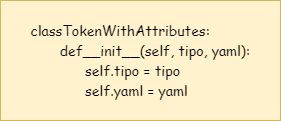
\includegraphics[scale=.8]{img4.png}
%\end{center}
%Por lo tanto ahora los elementos 'p', son del tipo TokkenWithAttributes.
%El atributo Tipo, es un string y el atributo 'Yaml' es una función que toma como %parámetro los tabs correspondientes a la posición del objeto actual.
%
%La estructura final del parser es:
%\begin{itemize}
%    \item Se generó el 'Parsing Tree'. $parsedValue = p[1]$
%    \item Se utilizó el atributo 'Yaml' del parsedValue, para imprimir la traducción. \\Este atributo es una función que toma por parámetro los tabs correspondientes al elemento actual. De esta manera se puede conseguir una simulación de nuestro requerimiento anterior para calcular los tabs de cada elemento aprovechando el parsing tree generado, sin crear un atributo 'heredado'.
%\end{itemize}

\section{Desiciones de diseño}
Para realizar la conversión de código JSON a YAML se precisó utilizar el estilo 'double-quoted', que conciste en explicitar el tipo string de una cadena agregándole comillas, ya que había 2 conflictos: 

\begin{itemize}
	\item \textbf{Cadenas de un tipo que podían confundirse con otro.} Por ejemplo, si se tiene la cadena $-$Cadena3 como clave de un objeto, a simple vista pareciera ser un item de un arreglo, cuando no lo es.
	\item \textbf{Otro conflicto se presenta cuando tenemos un catacter como '\texttt{\textbackslash n}',} ya que se necesita una representación para el salto de línea. Decidimos utilizar el estilo para la representación de todas las direcivas '\texttt{\textbackslash x}' ya que parece adecuado para la traducción.	
\end{itemize}

\section{Pruebas}

Se testeó el parser con los archivos \texttt{jasonObjet.txt},\texttt{jasonObjet1.txt},\texttt{jasonObjet2.txt} y \texttt{jasonObjet3.txt} consiguiendo los resultados deseados.
\begin{itemize}
\item \texttt{jasonObjet.txt} y \texttt{jasonObjet1.txt} contienen una cadena JSON válida cada uno
\item \texttt{jasonObjet2.txt} contiene una cadena JSON incompleta, por lo que su sintaxis es érronea
\item y \texttt{jasonObjet3.txt} contiene una cadena JSON con un objeto cuyas claves están repetidas.
\end{itemize}

\section{Requerimientos de Software}

Como se mencionó se usaron las siguientes herramientas:
\begin{itemize}
    \item Python, Version: 2.6
    \item PLY, Version: 3.5
\end{itemize}

\subsection{Comando de ejecución}
Para ejecutar el trabajo es necesario escribir por entrada standard un objeto JSON, por ejemplo:
\begin{center}
\begin{minipage}{0.8\textwidth}
	python3 tptleng.py $<$ jasonObjet.txt
\end{minipage}
\end{center}

\section{Referencias}
[-1-] Página:
\href{http://jsmachines.sourceforge.net/machines/lalr1.html}{LR Parser Table Generator}.

\end{document}
